\section{Method}
\label{sec:method}

\begin{figure*}
    \centering
   \resizebox{1.0\textwidth}{!}{%
    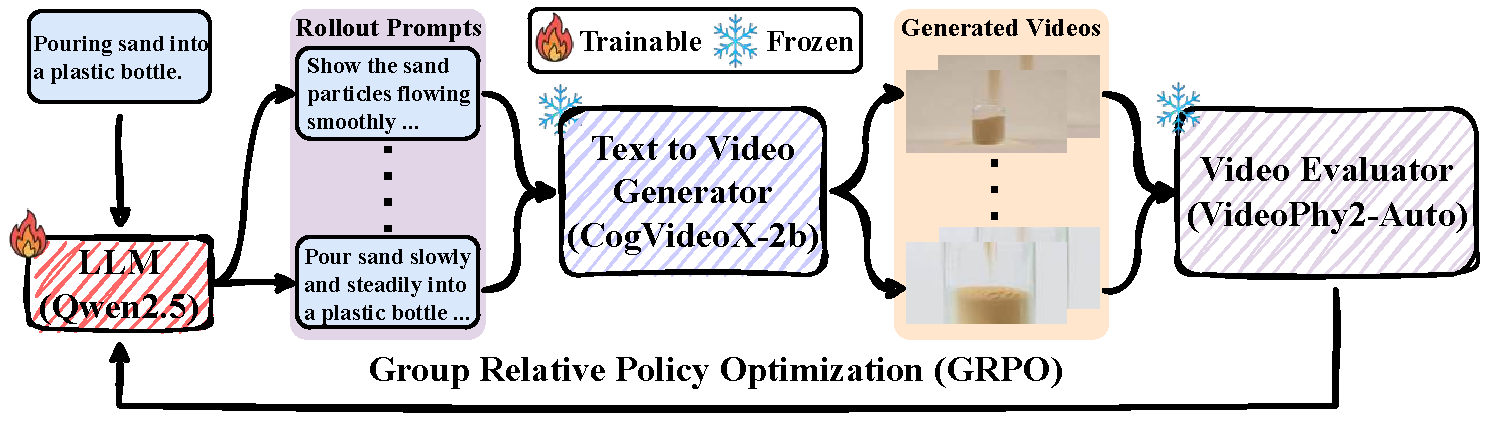
\includegraphics{figures/grpo.pdf}
    }
    \vspace{-0.1in}
    \caption{\textbf{PhyPrompt GRPO Pipeline.} For each input prompt, the LLM (Qwen2.5~\cite{Qwen2024}) generates multiple enhanced prompts and for each enhanced prompt, T2V generator (CogVideoX-2B~\cite{yang2024cogvideox}) generates one video. Video evaluator (VideoPhy2-Auto~\cite{bansal2025videophy2}) scores each video. We utilize GRPO to optimize the LLM.}
    \label{fig:pipeline}
    \vspace{-0.2in}
\end{figure*}

This section describes (i) our physics-focused Chain-of-Thought (CoT) dataset for supervised fine-tuning, (ii) GRPO-based prompt optimization, and (iii) our dynamic reward curriculum that resolves the inherent conflict between semantic fidelity and physical realism.

\subsection{Physics-Focused Chain-of-Thought Dataset}

We construct a CoT dataset to teach language models physics-aware prompt enhancement. Starting with 160 examples from PhyGenBench \cite{phygenbench2024}, each contains: an \emph{original prompt} $x$, an \emph{physical law} $L$, and an \emph{enhanced prompt} $y_{\text{GPT}}$ from GPT-4o \cite{achiam2023gpt-4o}. Since these lack explicit reasoning, we use GPT-4o1-preview \cite{jaech2024o1-preview} to generate step-by-step reasoning chains explaining how $x$ becomes $y_{\text{GPT}}$ via $L$.

The resulting dataset contains triplets $(x, \mathbf{r}, y_{\text{CoT}})$ where $\mathbf{r}$ is the reasoning chain and $y_{\text{CoT}}$ is the physics-aware prompt. This enables supervised fine-tuning of Qwen2.5 while preserving user intent.

\subsection{Two-Stage Training Pipeline}

\noindent\textbf{Supervised Fine-Tuning.} We initialize $\pi_{\theta}$ by minimizing cross-entropy loss:
\begin{equation}
  \mathcal{L}_{\text{SFT}}
  = -\E_{(x,y_{\text{CoT}})} \bigl[\log \pi_{\theta}(y_{\text{CoT}} \mid x)\bigr].
\end{equation}

\noindent\textbf{Reinforcement Learning via GRPO.} Figure~\ref{fig:pipeline} shows our pipeline. User prompt $x$ is rewritten by $\pi_{\theta}$ into enhanced prompt $y$, fed to a fixed T2V generator $G$ (CogVideoX-2B \cite{yang2024cogvideox}). The video $v = G(y)$ is scored by VideoPhy2-AutoEval \cite{bansal2025videophy2}, driving RL to refine $\pi_{\theta}$ without altering $G$.
For each prompt $x^{(j)}$ in batch size $B$, we sample $G=4$ candidate rewrites from $\pi_{\theta_{\text{old}}}$. Each yields video $v_i^{(j)} = G(y_i^{(j)})$ scored as $r_i^{(j)}$. Define group mean $\bar r^{(j)} = \frac{1}{G}\sum_{i=1}^G r_i^{(j)}$ and advantage:
\begin{equation}
  A_i^{(j)} = r_i^{(j)} - \bar r^{(j)}.
  \label{eq:advantage}
\end{equation}

We update $\pi_\theta$ via clipped GRPO loss with importance ratio
$w_i^{(j)} = \pi_{\theta}(y_i^{(j)}\mid x^{(j)})/\pi_{\theta_{\text{old}}}(y_i^{(j)}\mid x^{(j)})$:
\begin{align}
  \mathcal{L}_{\text{GRPO}}
  &= -\frac{1}{BG}\sum_{j=1}^B\sum_{i=1}^G
    \min\bigl(
      w_i^{(j)} A_i^{(j)}, \nonumber \\
    &\quad \text{clip}(w_i^{(j)}, 1-\epsilon, 1+\epsilon)\,A_i^{(j)}
    \bigr)
    + \beta\,D_{\mathrm{KL}}[\pi_{\theta_{\text{old}}}\|\pi_{\theta}],
\end{align}
where $\epsilon=0.2$ and $\beta$ weights KL divergence to the SFT initialization.

\subsection{Dynamic Multi-Objective Reward Design}

Semantic adherence (SA) and physical commonsense (PC) are inherently conflicting: single-objective optimization exhibits severe negative transfer where optimizing SA degrades PC and vice versa (Section~\ref{sec:reward_design}). Static weighted combinations cannot jointly maximize both objectives. We propose a dynamic reward curriculum that achieves synergistic optimization, exceeding the upper bounds of either single-objective approach.

\noindent\textbf{Reward Components.}
VideoPhy2-AutoEval \cite{bansal2025videophy2} provides two scores on a 1-5 Likert scale: \textbf{Semantic Adherence} ($r_{\text{sa}}$) measures video-prompt alignment, and \textbf{Physical Commonsense} ($r_{\text{pc}}$) measures physical plausibility.

\noindent\textbf{Dynamic Curriculum.}
The composite reward uses time-dependent weights:
\begin{equation}
  R(t) = w_{\text{sa}}(t) \cdot r_{\text{sa}} + w_{\text{pc}}(t) \cdot r_{\text{pc}},
  \label{eq:total_reward}
\end{equation}
with exponential decay:
\begin{equation}
  w_{\text{sa}}(t)=\exp\bigl(-\alpha\,t/T\bigr),\quad
  w_{\text{pc}}(t)=1-w_{\text{sa}}(t),
  \label{eq:weights}
\end{equation}
where $t$ is the training step, $T$ is total steps, and $\alpha$ controls decay rate.

\noindent\textbf{Compositional Learning Mechanism.}
Early training ($w_{\text{sa}} \approx 1$) establishes semantic scaffolding: object identities, relationships, and scene structure. Late training ($w_{\text{pc}} \approx 1$) refines this scaffolding with physical specificity: forces, dynamics, and causal interactions. This staged approach discovers prompt structures unreachable by single-objective optimization~\cite{bengio2009curriculum}.

Semantic grounding provides compositional scaffolding~\cite{scholkopf2021toward}, while physical constraints act as implicit regularization~\cite{liebel2018auxiliary}. SA-only optimization lacks refinement pressure from physics; PC-only optimization lacks semantic coherence to organize physical details. Our curriculum leverages both sequentially, achieving superadditive performance that simultaneously exceeds both single-objective upper bounds (in Section~\ref{sec:reward_design}). This demonstrates that our method discovers novel compositional prompt structures beyond static Pareto frontiers, aligning with recent multi-stage RL paradigms~\cite{guo2025deepseek} where progressive task decomposition unlocks capabilities beyond direct optimization.
